\documentclass{article}

\usepackage{amsmath}
\usepackage{amsfonts}
\usepackage{amssymb}
\usepackage{graphicx}
\usepackage{subcaption}
\usepackage[colorinlistoftodos]{todonotes}
\usepackage[colorlinks=true, allcolors=blue]{hyperref}

\usepackage{tikz}
\usetikzlibrary{positioning}
\usetikzlibrary{shapes,arrows}
\usepackage{adjustbox}
\tikzstyle{decision} = [diamond, draw, fill=blue!20,
        text width=4.5em, text badly centered, node distance=3cm, inner sep=0pt]
        \tikzstyle{block} = [rectangle, draw, fill=blue!20,
                text width=6em, text centered, rounded corners, minimum height=4em]
                \tikzstyle{line} = [draw, -latex']
                \tikzstyle{cloud} = [draw, ellipse,fill=red!20, node distance=3cm,
                        minimum height=2em]

\graphicspath{ {figures/} }

\usepackage{algorithm}
\usepackage[noend]{algpseudocode}

% Commands
\newcommand{\alphabet}{\mathcal{A}}

%EM Let's decide if we want to focus on generative model validation as a primary aim or as an application.
%EM One could imagine writing this either way-- the application would be "repertoires are complex. here's a bunch of summary statistics and a standard means of comparing them. one can use them to compare repertoires, be they simulated or real."
%BJO To me it seems that model validation provides a more substantive goal, but I'm willing to consider either option. Do you have a preference?
%EM I prefer having both.
\title{Immune receptor repertoire comparison and model validation via summary statistics}
\author{Branden Olson, Software WG folks, Frederick A Matsen IV}

\begin{document}

\maketitle

\begin{abstract}
The adaptive immune system generates an incredible diversity of antigen receptors to keep dangerous pathogens at bay.
The DNA sequences coding for these receptors arise by a complex process of random naive cell generation followed by a series of binding-based filters as well as (in the B cell case) affinity maturation, giving considerable structure to the distribution of sequences.
This structure leads to Rep-Seq datasets whose analysis is difficult but important for scientific understanding and public health applications.
One can compare these data sets to each other and to generative model simulations using summary statistics, or quantities that summarize some aspect of the repertoires.
In this paper we introduce \texttt{sumrep}, an R package that performs a wide variety of repertoire summaries and comparisons, and show how \texttt{sumrep} can be used to perform model validation.
We find regarding the summary statistics...
We find regarding the models...
\end{abstract}

\section*{Introduction}

B cells and T cells play critical roles in adaptive immunity through the cooperative identification of and response to antigens.
The sophisticated rearrangement of the genes that construct B cell receptors (BCRs) and T cell receptors (TCRs) allows for the recognition of a highly diverse set of antigen epitopes.
An individual's immune repertoire is the set of lymphocyte receptors present in the immune system and is constantly changing in time.

The random generation of immune repertoires from gene rearrangements invites probabilistic modeling and in particular model-based simulation.
In particular, it is natural to benchmark model-based inferential tools by applying them to simulations from the assumed model and assessing the performance.
Simulation tools can also be used to generate a null distribution to compare to data to look for a specific effect, such as natural selection \cite{Yaari2012-kk}.

To build and improve on such probabilistic frameworks, we must identify the strengths and limitations of the underlying models.
Statistical model validation compares features of simulated data to observed repertoire samples and evaluates their concordance (or lack thereof).
This is not as easy a task for repertoires as it is for other problems, where a model output may simply be a real number.
In contrast, repertoire models generate sets of nucleotide sequences that are sparse in the very large set of all possible nucleotide sequences.
Moreover, accurate repertoire models incorporate various underlying structures such as clonal family clusters or phylogenetic trees, further compounding the difficulties.
Indeed, immune repertoires are large, complex objects.

In such a setting, summary statistics are useful (and sometimes sufficient) for expressing discrepancies between model simulations and data, and also between simulations and between data sets.
Luckily, researchers have already derived many means of quantifying important features of repertoires.

These summary statistics can range from simple statistics such as the level of GC content, to statistics such as tree shapes which are applied to complex inferences.
Simple statistics acting on raw sequences are helpful because they are robust to potentially problematic assumptions of inferential methods as well as implementation intricacies.
For example, if our inferential method was linear regression, comparing fit slopes is less useful when the data is not close to a line, but comparing nonparametric statistics like the sample mean or range is still sensible.
On the other hand, statistics on the result of estimations are revealing when inferential model fit is reasonable, and can help reduce noise from sampling or measurement error.
In our linear regression example, comparing the general trends of points can be less distracted by noise than comparing the sets of points directly.

%EM This feels a bit out of place.
%BJO I think you added this a while back, but I tried to pad it with more context. Feel free to change or remove any part of it.
Still, determining how well a given summary can describe or distinguish a repertoire is a difficult task.
To illustrate, as noted above, BCR repertoires consist of collections of trees.
Thus, repertoires are substantially more complex than trees, and even for this strictly simpler problem there has been a lot of effort to define good summary statistics \cite{Mooers1997-jl}.
Tree statistics, albeit other ones, have also been a major focus of previous work in BCR sequence analysis \cite{Dunn-Walters2004-hv,Mehr2004-ej,Steiman-Shimony2006-fm,Shahaf2008-cc}.
These difficulties suggest that an eclectic approach using many summaries of diverse nature seems reasonable for a thorough view of a repertoire's characteristics.

[Cartoon of projecting repertoires in various directions into real space, and comparing the resulting projections?]

In this paper, we gather many summary statistics on repertoires and use them to perform model validation for state of the art simulation tools against real data.
We present \texttt{sumrep}, an R package that computes these summary distributions for Rep-Seq datasets and performs repertoire comparisons based on these summaries.
Furthermore, we investigate the effectiveness of various summary statistics in distinguishing between different observed repertoires as well as between simulated and observed data.
Although by comparing various generative models to real data, we obtain a validated means of generating data for benchmarking inferential tools, we don't do that here.
Also, although summary statistics can be used in simulation-based inferential methods such as approximate Bayesian computation, we don't do that here either.

\subsection*{Repertoire Comparison}

%EM This next paragraph doesn't feel abstract methods-y.
%BJO It may eventually be a better fit for a Discussion section, but I'll put it here for now.
Applications of a methodical lymphocyte repertoire comparison tool include:
\begin{itemize}
\item Comparing simulated repertoires to observed ones (model selection and validation)
\item Contrasting repertoires in the context of antigen response or vaccination design and evaluation
\item Assessing the performance of competing repertoire analysis tools
\item Evaluating artificial lymphocyte repertoires \cite{Finlay2012}
\end{itemize}

\section*{Methods}
\begin{table}
\makebox[\textwidth][c]{ % this centers a too-wide table
\begin{tabular}{c|c|c|c|c}
    Summary statistic & Annotations & Clustering & Phylogeny & Implementation
\\
\hline \hline
Pairwise distance matrix & No & No & No & \texttt{stringdist} \\
Distance to $k$th closest sequence & No & No & No & \texttt{stringdist} \\
GC-content & No & No & No & \texttt{ape} \\
Hot/cold spot motif frequencies & No & No & No & \texttt{Biostrings} \\
%BJO Hmm... we never really did much with this (i.e. the Eulerian path paper). Maybe we should discuss?
$k$mer frequency & No & No & No & -- \\
\hline
Distance from naive to mature & Yes & No & No & \texttt{stringdist} \\
%BJO Another one we kind of skipped over.
Distance to $k$th closest V-sequence & Yes & No & No & -- \\
CDR3 length & Yes & No & No & -- \\
Joint distribution of germline gene use & Yes & No & No & Custom \\
Levenshtein distance between CDR3s & Yes & No & No & \texttt{stringdist} \\
Hydrophobicity & Yes & No & No & \texttt{Peptides} \\
Atchley factors & Yes & No & No & \texttt{HDMD} \\
Aliphatic index & Yes & No & No & \texttt{Peptides} \\
G.R.A.V.Y. index & Yes & No & No & \texttt{alakazam} \\
Per-gene substitution rate & Yes & No & No & Custom \\
Per-gene-per-position substitution rate & Yes & No & No & Custom \\
Per-base mutability model & Yes & No & No & \texttt{shazam} \\
Per-base substitution model & Yes & No & No & \texttt{shazam} \\
%BJO This one doesn't depend on fit-star, right?
%EM Yes, but we could just count Ts vs Tv, call it a "ratio" and drop the model-based rigor.
Transition/transversion rates & Yes & No & No & -- \\
Positional distance between mutations & Yes & No & No & Custom \\
Distance from naive to mature & Yes & No & No & \texttt{stringdist} \\
V/D/J deletion/insertion lengths & Yes & No & No & -- \\
Transition matrix for insertions & Yes & No & No & Custom \\
\hline
Cluster size distribution & Yes & Yes & No & Custom \\
Hill numbers (diversity indices) & Yes & Yes & No & \texttt{alakazam} \\
Selection estimates & Yes & Yes & No & \texttt{shazam} \\
%BJO blocked due to fit-star
Transition/transversion rates & Yes & Yes & No & -- \\
\hline
Sackin index & Yes & Yes & Yes & \texttt{CollessLike} \\
Colless-like index & Yes & Yes & Yes & \texttt{CollessLike} \\
Cophenetic index & Yes & Yes & Yes & \texttt{CollessLike} \\
%BJO To be delineated
Graph-theoretical features & Yes & Yes & Yes & -- \\
\end{tabular}
}
\caption{Working table of summary statistics as well as their respective levels of assumed post-processing.}
\label{tab:SummaryStatistics}
\end{table}

%EM This should be expanded. E.g. to drive home that we need to use partis or some such tool.
Table \ref{tab:SummaryStatistics} lists the summary statistics currently supported by \texttt{sumrep}, and includes the assumed level of annotation, clustering, and phylogenetic inference.
The first group does not require any post-processing and are completely tool-independent.
The second group requires standard sequence annotations, such as inferred naive ancestor sequences, germline gene assignments, and indel information.
The third group also requires clonal family cluster assignments.
The fourth group further requires an imputed phylogeny for each clonal family.
\texttt{sumrep} itself does not perform any annotation, clustering, or phylogeny inference, but rather assumes such metadata have been pre-computed and included in the given dataset; in principle, one can use any tool which performs these tasks as expected.

Other possible statistics:

\begin{itemize}
\item Clustered sequences: estimated total diversity reviewed in \cite{Mehr2012-se}
\item Trees: graph theoretical features \cite{Dunn-Walters2002-cu,Dunn-Walters2004-hv,Mehr2004-ej,Shahaf2008-cc,Budeus2015-ab,Yaari2015-ss}.
Applied to make inferences about data \cite{Steiman-Shimony2006-fm}.
\item Trees + sequence level information for selection estimates \cite{Uduman2014-pb}
\end{itemize}


\subsection*{Divergence}
The general approach of \texttt{sumrep} is to get distributions of a given summary statistic for the two repertoires in consideration and compare them via some metric or divergence.
We have elected to use Jenson-Shannon divergence for most of our comparison functions.
The Jenson-Shannon divergence of probability distributions $P$ and $Q$ with densities $p(\cdot)$ and $q(\cdot)$ is a symmetrized Kullbeck-Leiber divergence, defined as
\begin{equation}
\text{JSD}\left(P || Q\right) := \frac{\text{KLD}\left(P || M\right) + \text{KLD}\left(Q || M\right)}{2}
\end{equation}
where $M := (P + Q)/2$ and $\text{KLD}(P || M)$ is the usual KL-divergence,
\begin{equation}
\text{KLD}\left(P_1 || P_2\right) := \operatorname{E}_{\mathbf X \sim P_1}\left[ \log\left(\frac{p_1(\mathbf X)}{p_2(\mathbf X)}\right) \right].
\end{equation}
In the case where $P$ and $Q$ are both discrete distributions, this becomes
\begin{equation}
\text{KLD}\left(P_1 || P_2\right) = \sum_{n \in \Omega} p_1(n) \log\left( \frac{p_1(n)}{p_2(n)} \right)
\end{equation}
where $\Omega$ is the countable sample space for $P_1$.
Because the discrete formulation is much nicer to worth with than the continuous one, we discretize continuous samples and treat them as discrete data.
By default, we use $B = \max\left(\left\lceil \sqrt{\min(m, n)} \right \rceil, 2\right)$ bins of equal length, which scales reasonably with $m$ and $n$ simultaneously.
Instead of binning, one could construct approximating functions for the two densities and compute the expectation via numerical integration; this may increase accuracy but also introduces extra complexity and possible division-by-zero issues.

Sometimes it makes more sense to use other distance metrics, such as the sum of absolute differences for count data:
%EM I prefer equations to have an eq: label, figures a fig: label, etc.
\begin{equation}\label{eq:SAD}
    d(R_1, R_2; c, \mathcal S) = \sum_{s \in \mathcal S} \left| c(s; R_1) - c(s; R_2) \right|.
\end{equation}
In words, \eqref{eq:SAD} iterates over each element $s$ in some set $\mathcal S$, calculates the count $c$ of $s$ within repertoires $R_1$ and $R_2$ respectively, takes the absolute difference of counts, and appends this to a rolling sum.
This metric is well suited for comparing joint V/D/J-gene usage distributions:
if $\mathcal V$, $\mathcal D$, and $\mathcal J$ represent the germline sets of V, D, and J genes, respectively,
defining define usage $u$ of gene triple $(v, d, j) \in \mathcal V \times \mathcal D \times \mathcal J$ for repertoire $R$ as
\begin{equation}
u(R; v, d, j) = \#\left\{s \in R: s_v = v \land s_d = d \land s_j = j\right\},
\end{equation}
then our comparison metric of joint VDJ gene usage for repertoires $R_1$ and $R_2$ becomes
\begin{equation}
d(R_1, R_2; u, \mathcal V, \mathcal D, \mathcal J) = \sum_{v \in \mathcal V} \sum_{d \in \mathcal D} \sum_{j \in \mathcal J} \left| u(v, d, j; R_1) - u(v, d, j; R_2) \right|.
\end{equation}

\subsection*{Efficient computation by subsampling and averaging}
Computing full summaries can be computationally inefficient for even moderately sized repertoires.
When the target summary is a distribution, we can gain efficiency by subsampling and averaging.
%EM I like to caps Algorithm, Figure, etc, and add ~ between for a non-breaking space. I didn't make changes below.
This idea is laid out in Algorithm~\ref{DivergenceAveraging}, which uses a rolling average to update the estimated divergence by computing the divergence from subsamples of the two distributions.
Algorithm~\ref{DivergenceAveraging} is automatic in that it converges when standardized successive divergence estimates are sufficiently close.

\begin{algorithm}
    \caption{Compute automatic approximate divergence.\\
    \textbf{Input:} distributions $P$ and $Q$, divergence function $D$, subsample size $m$, convergence tolerance $\varepsilon$\\
    \textbf{Output:} approximate $D$-divergence between $P$ and $Q$
    }
    \label{DivergenceAveraging}
    \begin{algorithmic}
    \State $n \gets 0$;
    \State error $\gets \infty$;
    \While{error $> \varepsilon$}:
    \State $p_n \gets \text{subsample}(P, m)$
    \State $q_n \gets \text{subsample}(Q, m)$
    \State $D_n(P, Q) \gets D(p_n, q_n)$
    %EM This is sad when n=0.
    \State $\overline{D}_n \gets \frac{(n - 1) \overline{D}_{n-1}(P, Q) + D_n(P, Q)}{n}$;
    \State error $\gets \frac{ \left| \overline D_n(P, Q) - \overline D_{n-1}(P, Q) \right|}
        { \overline D_n(P, Q) }$
    \State $n \gets n + 1$
    \EndWhile
    \Return $D_n(P, Q)$
\end{algorithmic}
\end{algorithm}


When the summary distributions themselves are of interest, we can apply the same reasoning for approximating them.
Algorithm~\ref{DistributionAveraging} describes an automatic procedure to approximate a distribution $d$.
Here, the idea is to keep appending subsamples of $d$ to a working approximation until successive iterates have a sufficiently small JS-divergence.
\begin{algorithm}
    \caption{Compute automatic approximate distribution.\\
        \textbf{Input:} distribution $d$, subsample size $m$, convergence tolerance $\varepsilon$\\.
        \textbf{Output:} subsampled approximation to $d$}
    \label{DistributionAveraging}
    \begin{algorithmic}
        \State $d_0 \gets \text{subsample}(d, m)$
        \State $n \gets 1$
        \State error $\gets \infty$
        \While{error $> \varepsilon$}:
        \State $d_\text{samp} \gets \text{subsample}(d, m)$
        \State $d_n \gets \text{concatenate}(d_{n-1}, d_\text{samp})$
        \State error $\gets \text{JSD}(d_{n-1}, d_n)$
        \State $n \gets n + 1$
        \EndWhile
    \end{algorithmic}
    \Return $d_n$

\end{algorithm}

\subsection*{Scoring summary statistic replication by model}
%EM Would it be worth using some of these figures https://github.com/matsen/talks/tree/gh-pages/figures/sumrep ? (I just invited you.) I think that we're used to this framework but it may be a little strange for others.
We would like a measure of how well a statistic is replicated when a model performs simulations using parameters infered from the observed repertoire dataset.
One approach is to score the statistic $s$ based on the average divergence of observations to their simulated counterparts, and the average divergence of observations and other observations.
Let $\mathcal I$ be the set of dataset indices so that each separate dataset for a (individual, timepoint) pair corresponds to a unique index.
Furthermore, let $R_{i, \text{obs}}$ and $R_{i, \text{sim}}$ be the $i$th observed and simulated repertoire, respectively, and $\mathcal D(R_1, R_2; s)$ be the divergence of repertoires $R_1$ and $R_2$ based on statistic $s$, we have
\begin{equation}
    \text{score}(s) := \log \left( \frac{ \frac{1}{|\mathcal I|} \sum_{i \in \mathcal I} \mathcal D \left( R_{i, \text{obs}}, R_{i, \text{sim}} ; s\right) }
    { \frac{1}{\frac{1}{2} |\mathcal I|\left(|\mathcal I| - 1\right)}
        \sum_{\substack{i, j \in \mathcal I \\ i \ne j}} \mathcal D\left(R_{i, \text{obs}}, R_{j, \text{obs}}; s\right) } \right)
\end{equation}

\section*{Results}

%EM I suggest having the first section of the results be a short blurb about the R package.

%EM Then a section heading about model validation here.

%EM I suggest moving this to "methods"-- it describes the "materials" used for your analysis.
%EM We need a little more intro here to say that we're using the flu dataset etc.
Table \ref{tab:Datasets} gives metadata for each dataset used in this section.
\begin{table}
\begin{tabular}{c|c|c|c|c|c}
	Dataset label & Dataset type & Annotation tool & Germline set & Individual & Time point \\
	\hline
    \texttt{p\_f1} & Observation &     \texttt{partis} & \texttt{partis} & F & 1 hour \\
    \texttt{p\_f2} & Observation &     \texttt{partis} & \texttt{partis} & F & 8 days \\
    \texttt{p\_g1} & Observation &     \texttt{partis} & \texttt{partis} & G & 1 hour \\
    \texttt{i\_f1} & Observation &     \texttt{igblast} & \texttt{partis} & F & 1 hour \\
    \texttt{i\_f2} & Observation &     \texttt{igblast} & \texttt{partis} & F & 8 days \\
    \texttt{i\_g1} & Observation &     \texttt{igblast} & \texttt{partis} & G & 1 hour\\
    \texttt{pi\_f1} & Observation &    \texttt{partis} & \texttt{igblast} & F & 1 hour\\
    \texttt{pi\_f2} & Observation &    \texttt{partis} & \texttt{igblast} & F & 8 days\\
    \texttt{pi\_g1} & Observation &    \texttt{partis} & \texttt{igBlast} & G & 1 hour\\
    \texttt{p\_f1\_sim} & Simulation & \texttt{partis} & \texttt{partis} & F & 1 hour\\
    \texttt{p\_f2\_sim} & Simulation & \texttt{partis} & \texttt{partis} & F & 8 days\\
    \texttt{p\_g1\_sim} & Simulation & \texttt{partis} & \texttt{partis} & G & 1 hour\\
    \texttt{pi\_f1\_sim} & Simulation& \texttt{partis} & \texttt{igblast} & F & 1 hour\\
    \texttt{pi\_f2\_sim} & Simulation& \texttt{partis} & \texttt{igblast} & F & 8 days\\
    \texttt{pi\_g1\_sim} & Simulation& \texttt{partis} & \texttt{igblast} & G & 1 hour\\
\end{tabular}
\caption{Dataset notation.}
\label{tab:Datasets}
\end{table}
In short, the notation is as follows.
A prefix of \texttt{p} corresponds to \texttt{partis} annotations, a prefix of \texttt{i} corresponds to \texttt{igblast} annotations, and a prefix of \texttt{pi} corresponds to \texttt{partis} annotations using the default \texttt{igblast} germline databases;
this is followed by a letter representing the individual succeeded by a number corresponding to the time point;
finally, we append the \texttt{sim} suffix if the dataset was simulated from an individual's inferred model parameters.

\subsection*{Comparing observations to model simulations per model}
%EM I suggest this is more methods
In this section we perform model validation on the BCR sequence annotation and clonal family clustering strategy implemented in \texttt{partis}\cite{Ralph2016-nw, Ralph2016-iz}.
We compute each summary statistic listed in table \ref{tab:SummaryStatistics} for each dataset in table \ref{tab:Datasets}.
Since \texttt{partis} returns a list of the top most probable scenarios for each rearrangement event, we use only the most likely for each sequence.
%EM cft package is going to get us in trouble-- best to just describe the alignment and tree building programs (with versions)
For those statistics which require an inferred phylogenetic tree, we use the cft package with the \texttt{partis}-partitioned data as input.
Then, we compute the comparisons or divergences between each observed-simulated pair as well as between each of the observed datasets.
Figure \ref{PartisWorkflow} describes the workflow of this procedure for a given dataset.
\begin{figure}
\begin{adjustbox}{max totalsize={\textwidth}{.5\textheight},center}
    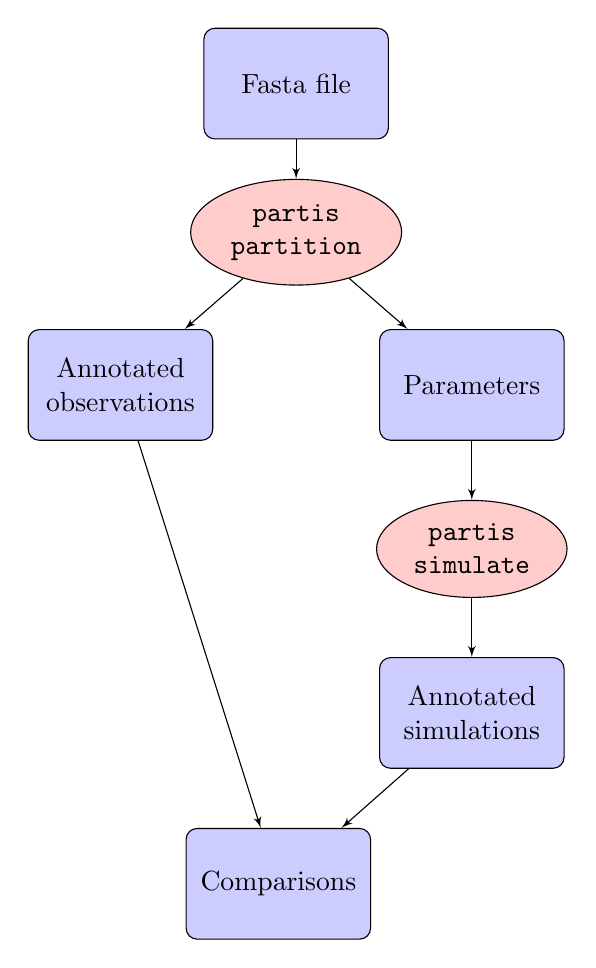
\begin{tikzpicture}
        \node[block](fasta){Fasta file};
        \node[cloud, below =0.5 cm of fasta, align=center](partis){\texttt{partis}\\ \texttt{partition}};

        \node[block, below left=0.75 cm and 0.1 cm of partis](partisdata){Annotated observations};
        \node[block, below right=0.75 cm and 0.1 cm of partis](params){Parameters};

        \node[cloud, below=0.75cm of params, align=center](simulate){\texttt{partis} \\ \texttt{simulate}};

        \node[block, below = 0.75cm of simulate](sim){Annotated simulations};


        \node[block, below left=0.75 and 0.1cm of sim](c1){Comparisons};

        \path[line](fasta) -- (partis);

        \path[line] (partis) -- (partisdata);
        \path[line] (partis) -- (params);


        \path[line] (params) -- (simulate);
        \path[line] (simulate) -- (sim);

        \path[line] (partisdata) -- (c1);
        \path[line] (sim) -- (c1);

    \end{tikzpicture}
\end{adjustbox}
\caption{Workflow for comparing a given observed repertoire dataset to an example simulated dataset via \texttt{partis}.}
\label{PartisWorkflow}
\end{figure}

%EM Results paragraphs concern what was found. Can you comment on overall trends or interesting things we found that people can find in the figure?
Figure \ref{SimObs} displays the divergences of each statistic in \ref{tab:SummaryStatistics} for three observed repertoires.
\begin{figure}
    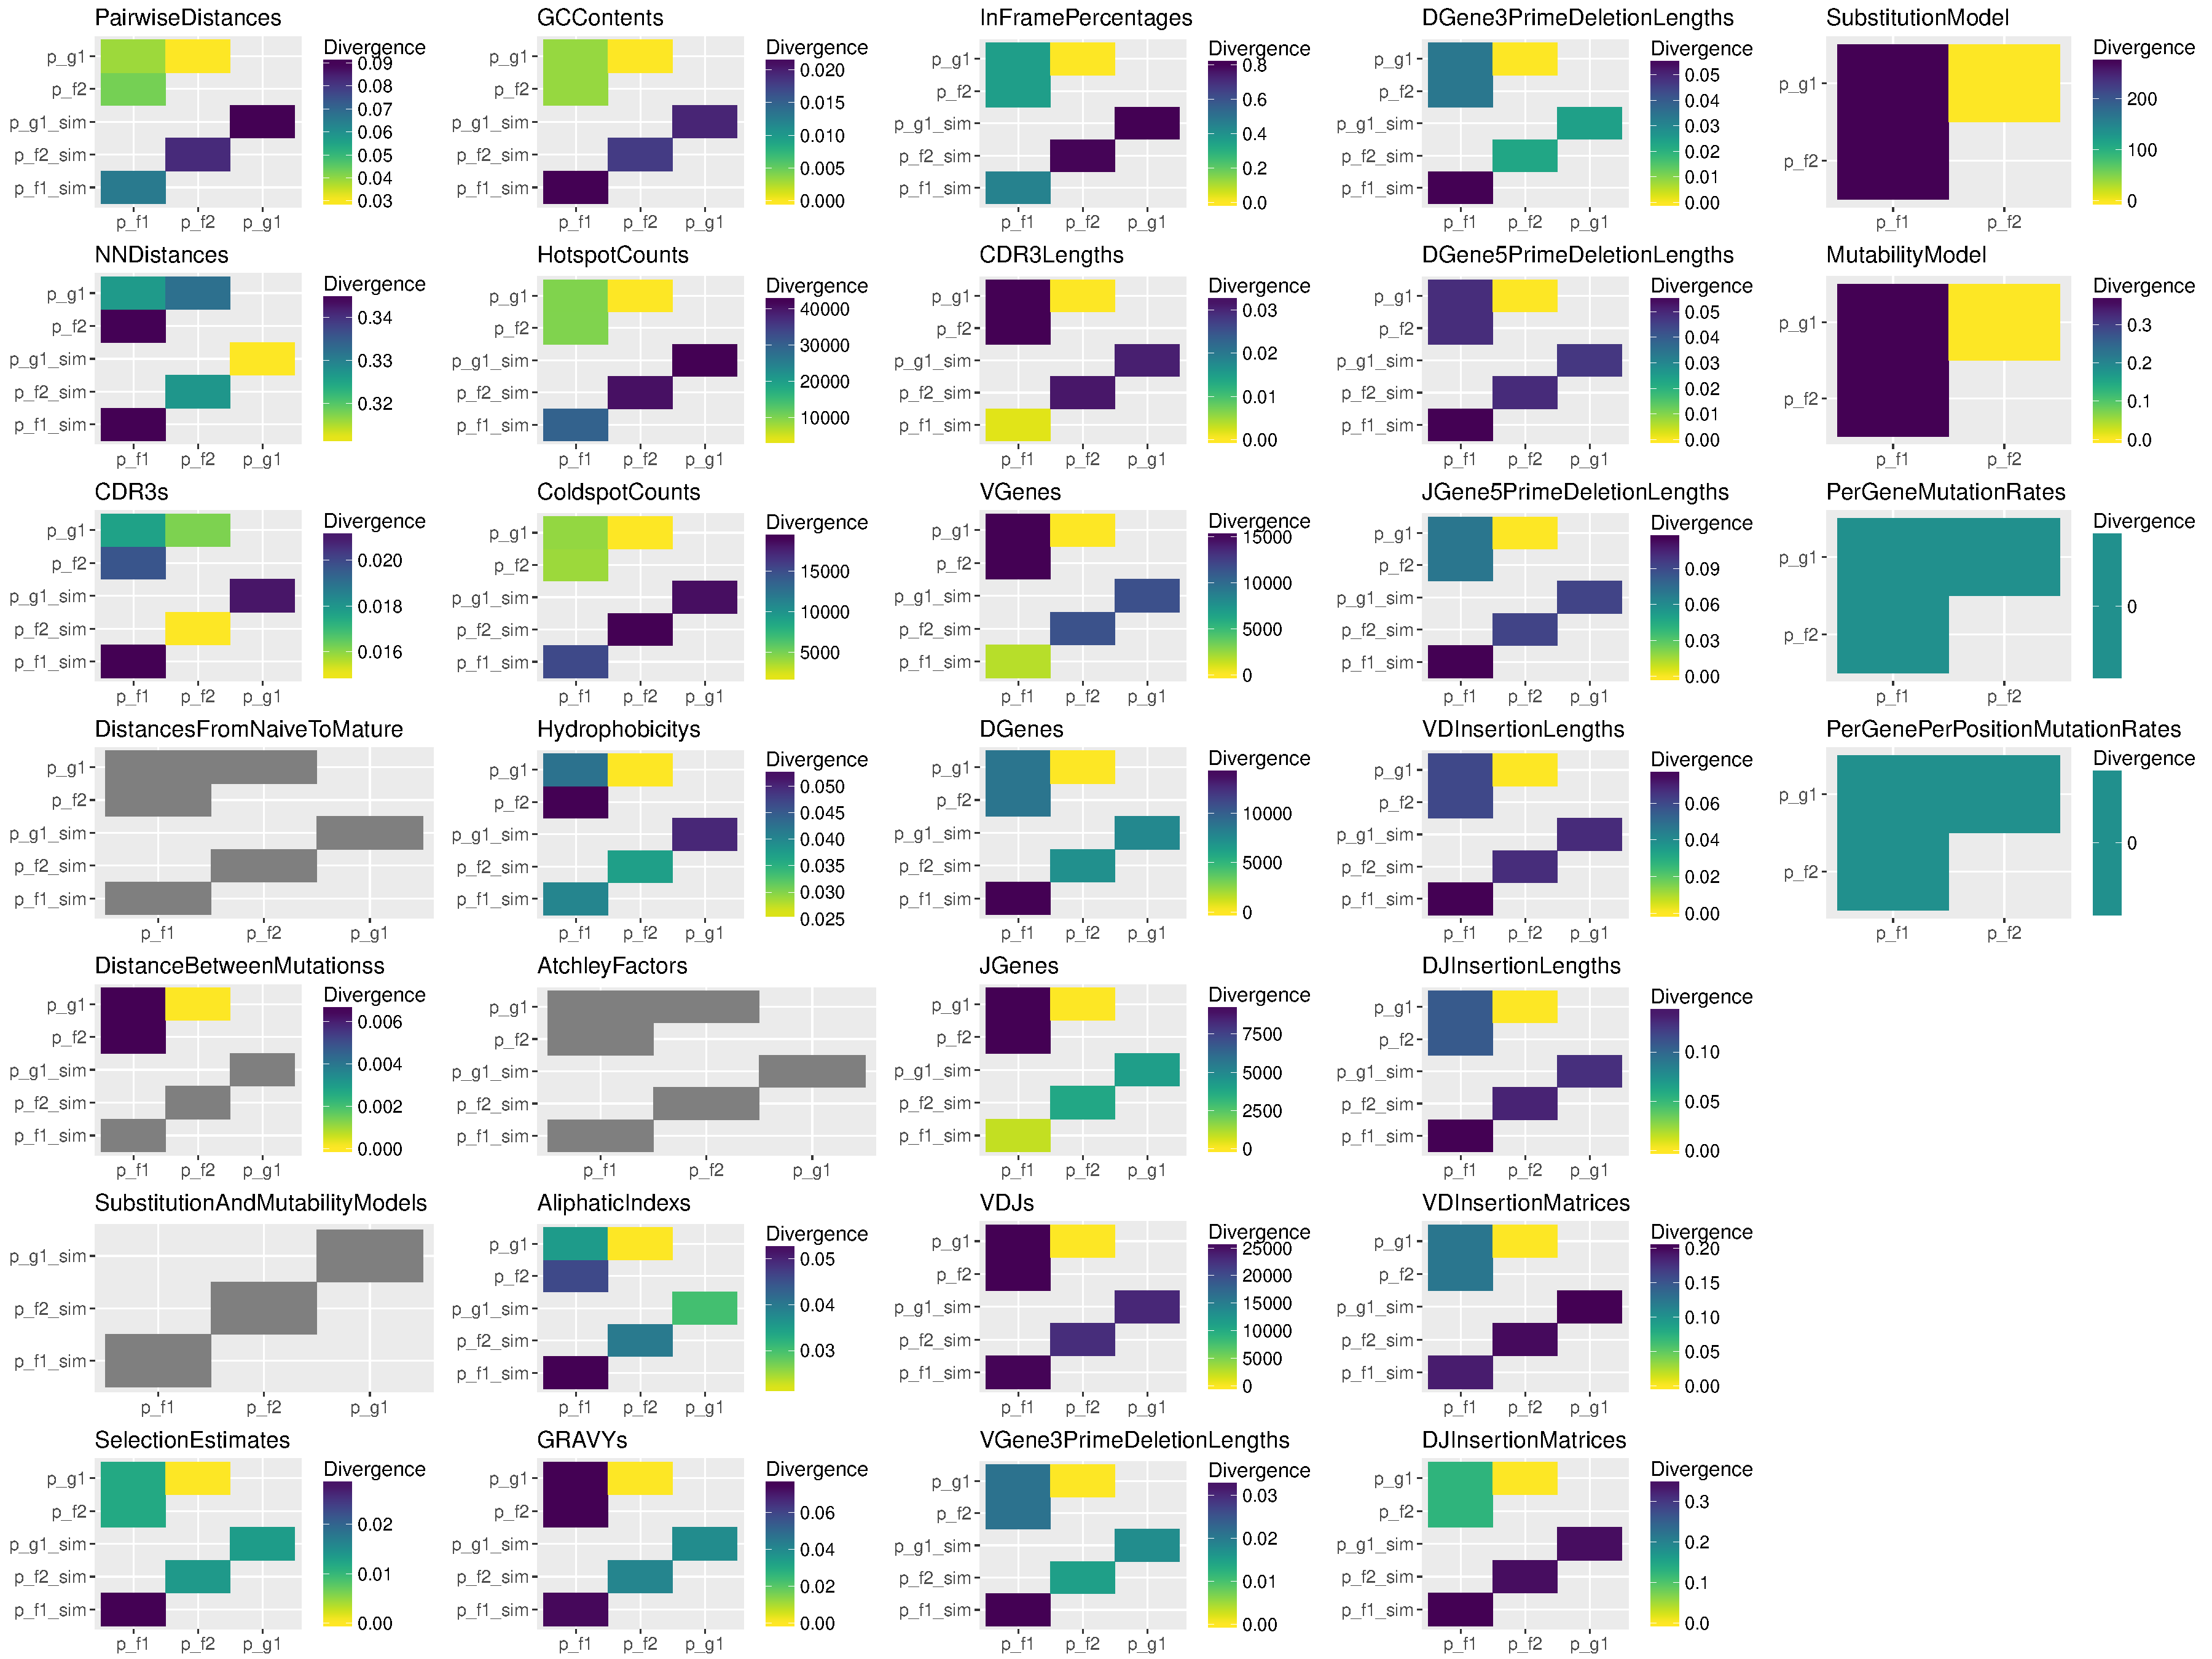
\includegraphics[width=\linewidth]{Figures/sim_obs.pdf}
    \caption{Divergences of empirical summary distributions based on three individual observed datasets.}
    \label{SimObs}
\end{figure}
Because the absolute divergence values are sensitive to scale as well as the type of divergence used, we also include divergences for each observation-observation pair as a benchmark.
The idea here is that a very good simulator should result in low divergence values between its reference repertoire and its simulated repertoire, as opposed to comparing the observed dataset to any other dataset.
For such a simulator, the diagonal at the bottom of the plots in figure \ref{SimObs}, which represents observation-simulation divergences, would have lighter colors than those in the upper left corner, which represent observation-observation divergenes.
In reality, it tends to be the case that observed repertoires are more similar to each other than an observed repertoire is to its simulated counterpart.

A valid concern about our methodology is that \texttt{partis} simulations would be unreasonably biased by \texttt{partis} annotations on which they are based.
To address this, we performed dataset annotation using standalone \texttt{igblast} \cite{Ye2013-kl}, and compared these to simulations based on \texttt{partis} annotations using the \texttt{igblast} germline databases.
Change-O was used to parse the \texttt{igblast} output \cite{Gupta2015-iu}.
Our strategy is analogous to the one above but with the inclusion of a separate path for \texttt{igblast} annotations.
The workflow for this procedure is displayed in figure \ref{IgblastWorkflow}.
\begin{figure}
    \begin{adjustbox}{max totalsize={\textwidth}{.8\textheight},center}
        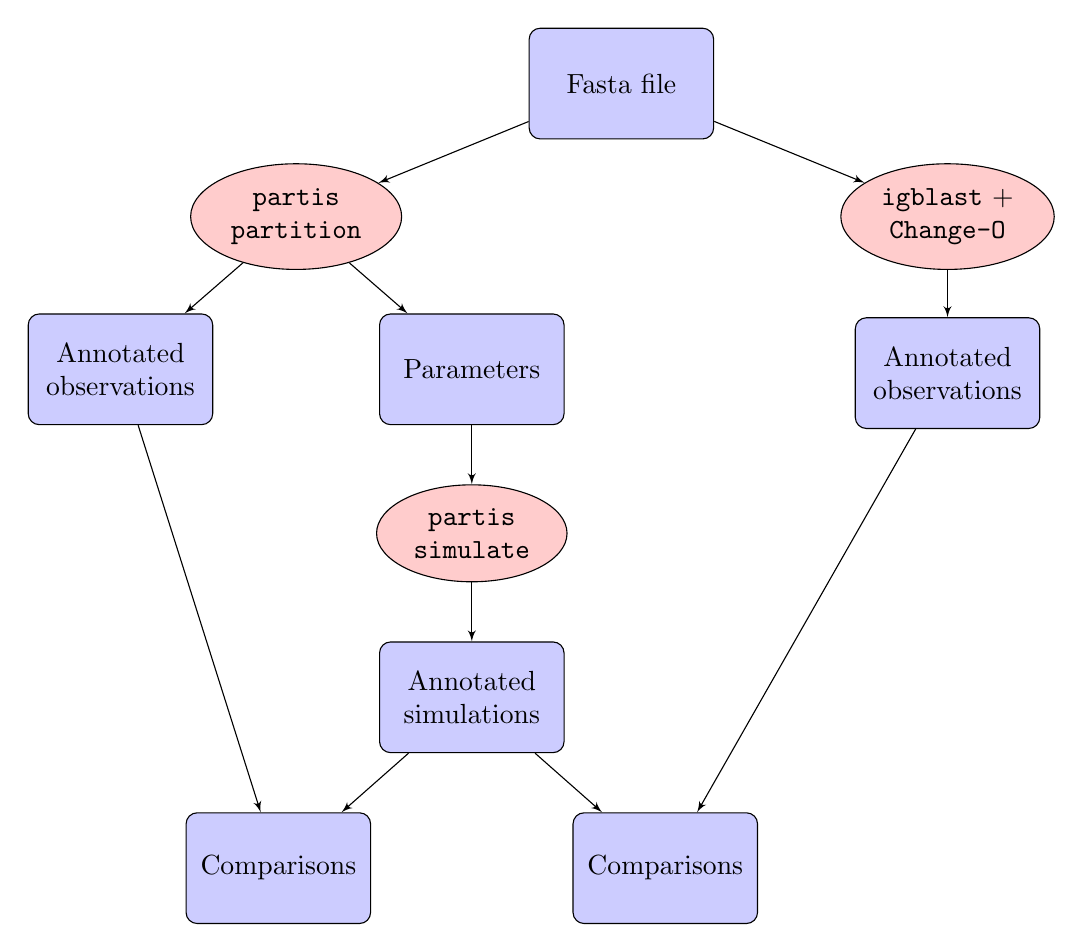
\begin{tikzpicture}
            \node[block](fasta){Fasta file};
            \node[cloud, below left=0.5 cm and 2 cm of fasta, align=center](partis){\texttt{partis}\\ \texttt{partition}};
            \node[cloud, below right=0.5 cm and 2 cm of fasta, align=center](igblast){\texttt{igblast} + \\ \texttt{Change-O}};

            \node[block, below left=0.75 cm and 0.1 cm of partis](partisdata){Annotated observations};
            \node[block, below right=0.75 cm and 0.1 cm of partis](params){Parameters};

            \node[cloud, below=0.75cm of params, align=center](simulate){\texttt{partis} \\ \texttt{simulate}};

            \node[block, below = 0.75cm of simulate](sim){Annotated simulations};

            \node[block, below=0.6 cm of igblast](igblastdata){Annotated observations};

            \node[block, below left=0.75 and 0.1cm of sim](c1){Comparisons};
            \node[block, below right=0.75 and 0.1cm of sim](c2){Comparisons};

            \path[line](fasta) -- (partis);
            \path[line](fasta) -- (igblast);

            \path[line] (partis) -- (partisdata);
            \path[line] (partis) -- (params);

            \path[line] (igblast) -- (igblastdata);

            \path[line] (params) -- (simulate);
            \path[line] (simulate) -- (sim);

            \path[line] (partisdata) -- (c1);
            \path[line] (sim) -- (c1);

            \path[line] (igblastdata) -- (c2);
            \path[line] (sim) -- (c2);
        \end{tikzpicture}
    \end{adjustbox}
    \caption{Workflow for comparing \texttt{partis} and \texttt{igblast} annotations to partis simulations}
    \label{IgblastWorkflow}
\end{figure}
The results are displayed in figure \ref{PartisIgb}.
\begin{figure}
    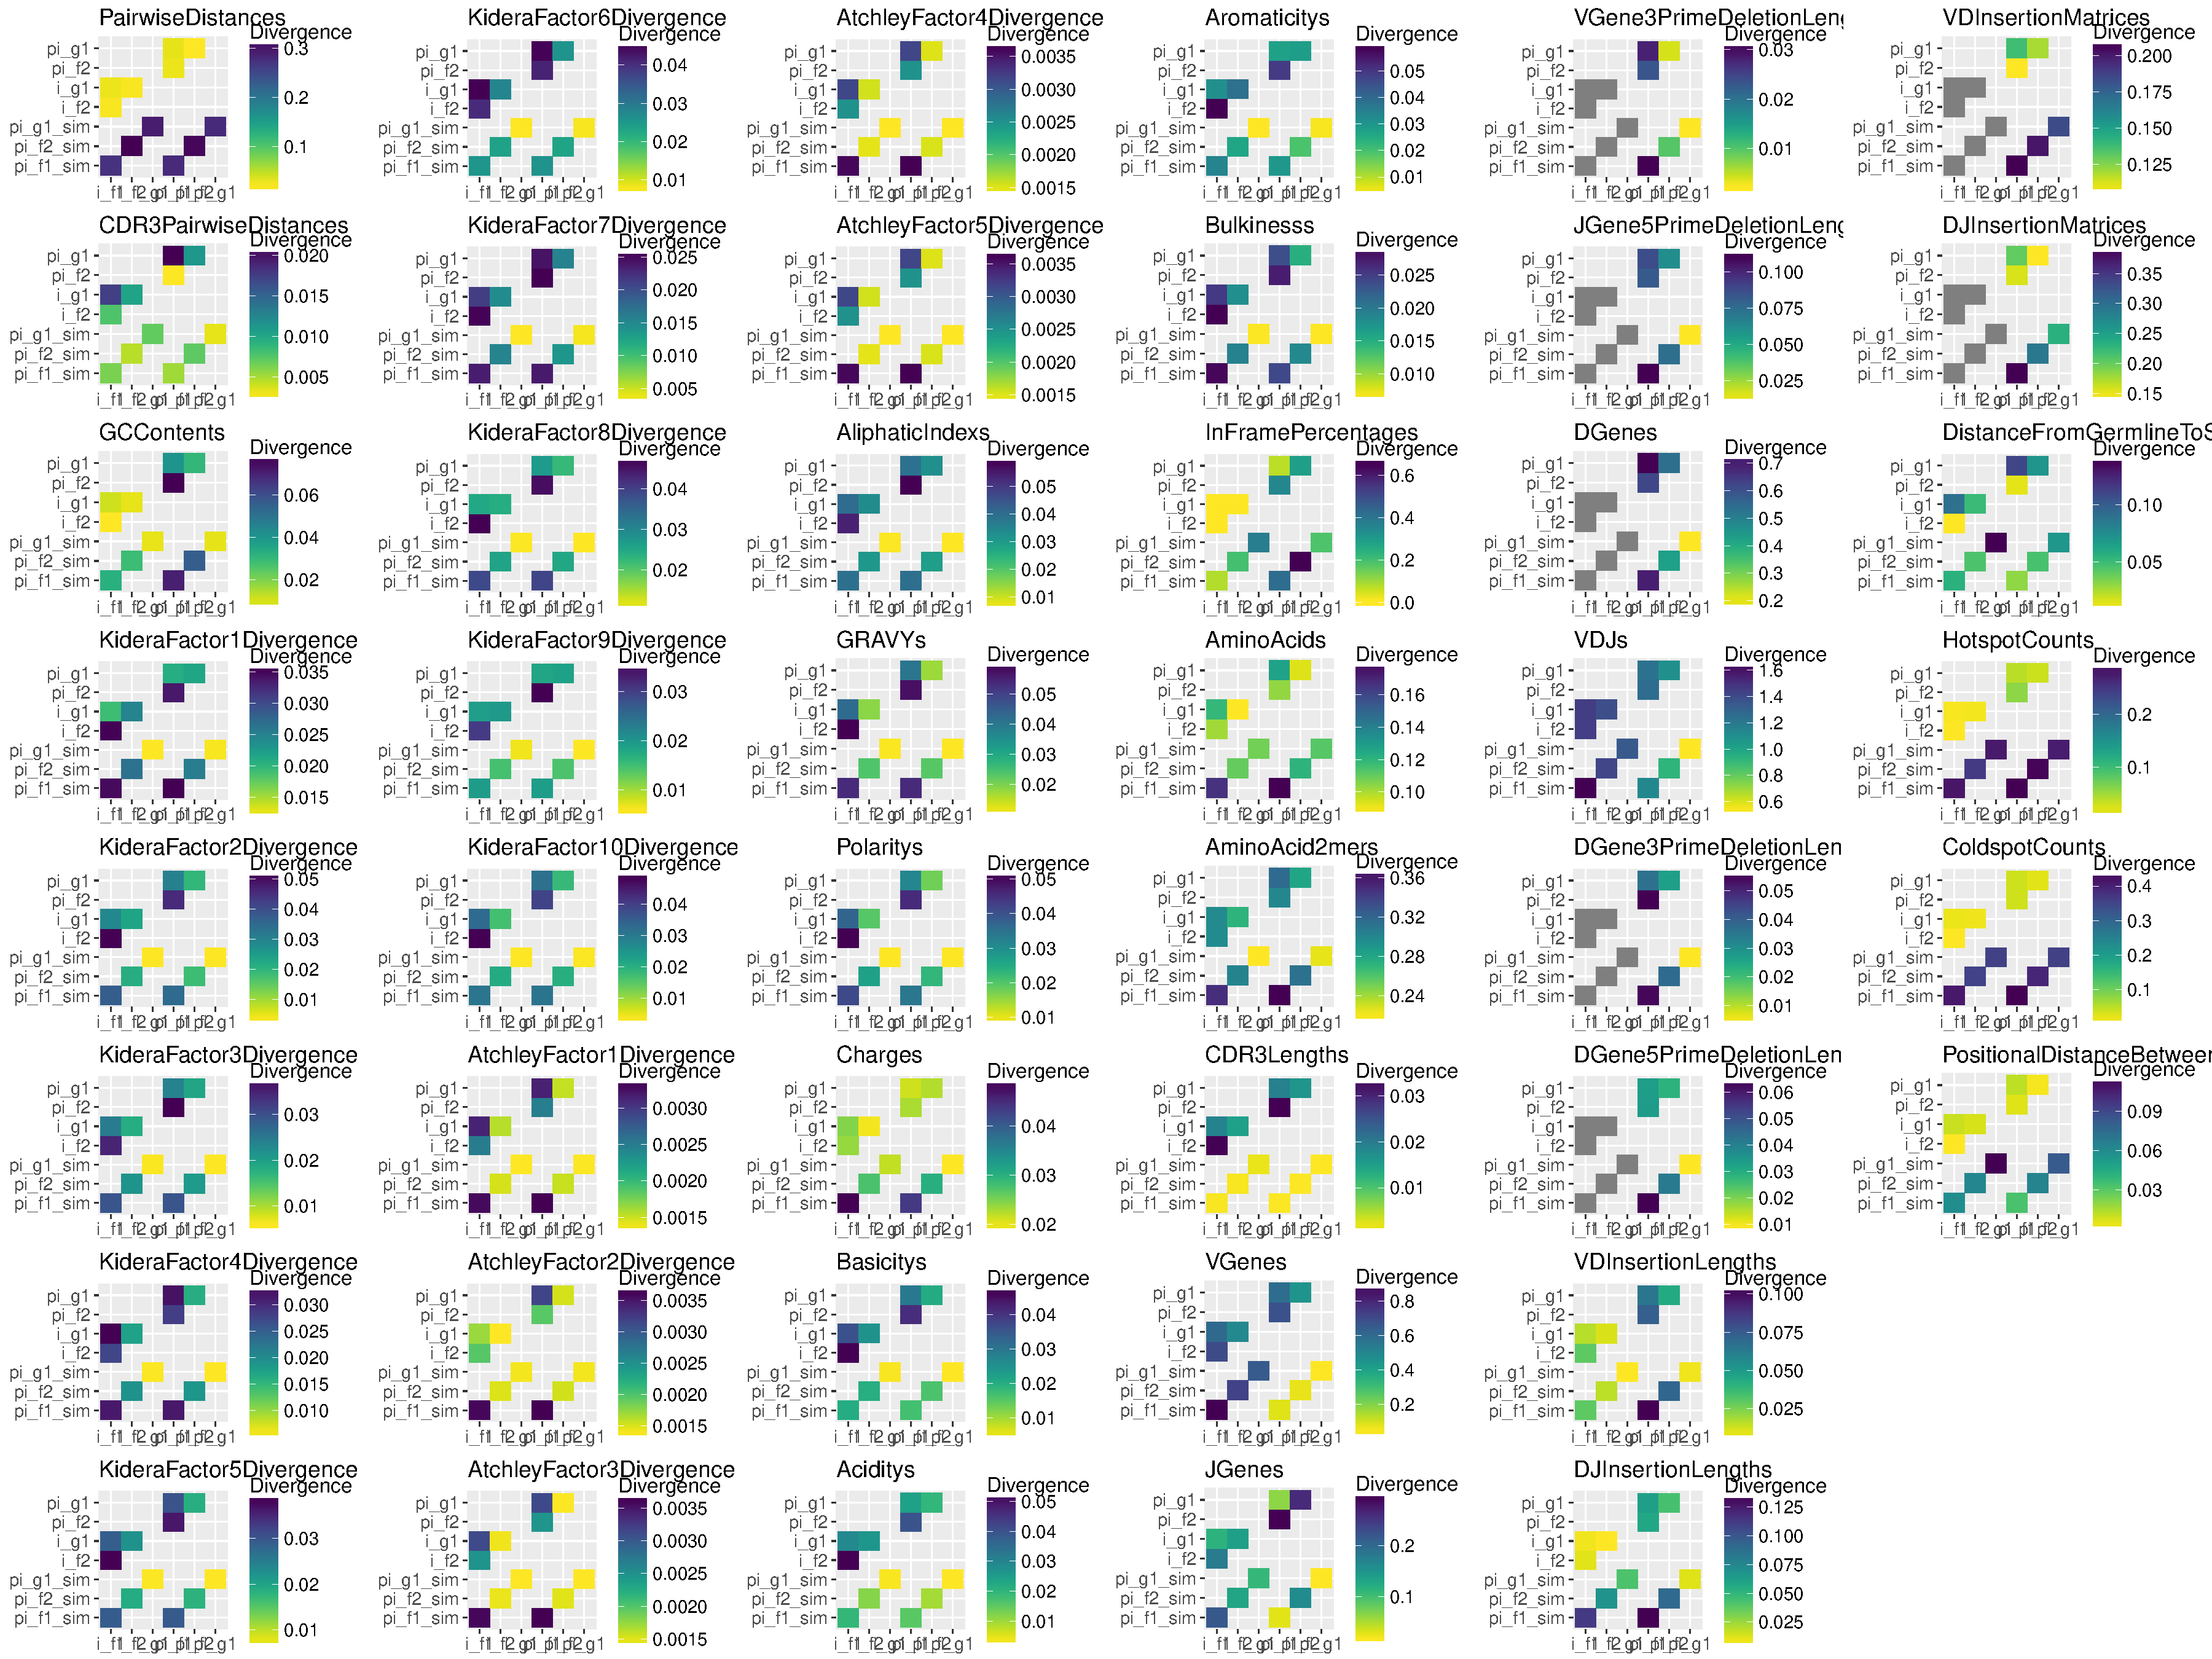
\includegraphics[width=\linewidth]{Figures/partis_igb.pdf}
    \caption{Comparing divergences for \texttt{igblast} annotations and \texttt{partis} simulations based on the same individual observed repertoires.
        We use the default germline databases in \texttt{igblast} for consistency.
    }
    \label{PartisIgb}
\end{figure}
The plots do not suggest any systematic bias in our approach.


\subsection*{Assessing summary statistic replication by model}
%EM Need some text here describing what was found.
Figure \ref{Scores} displays the LRD scores for the three individuals based on \texttt{partis} simulations.
\begin{figure}
    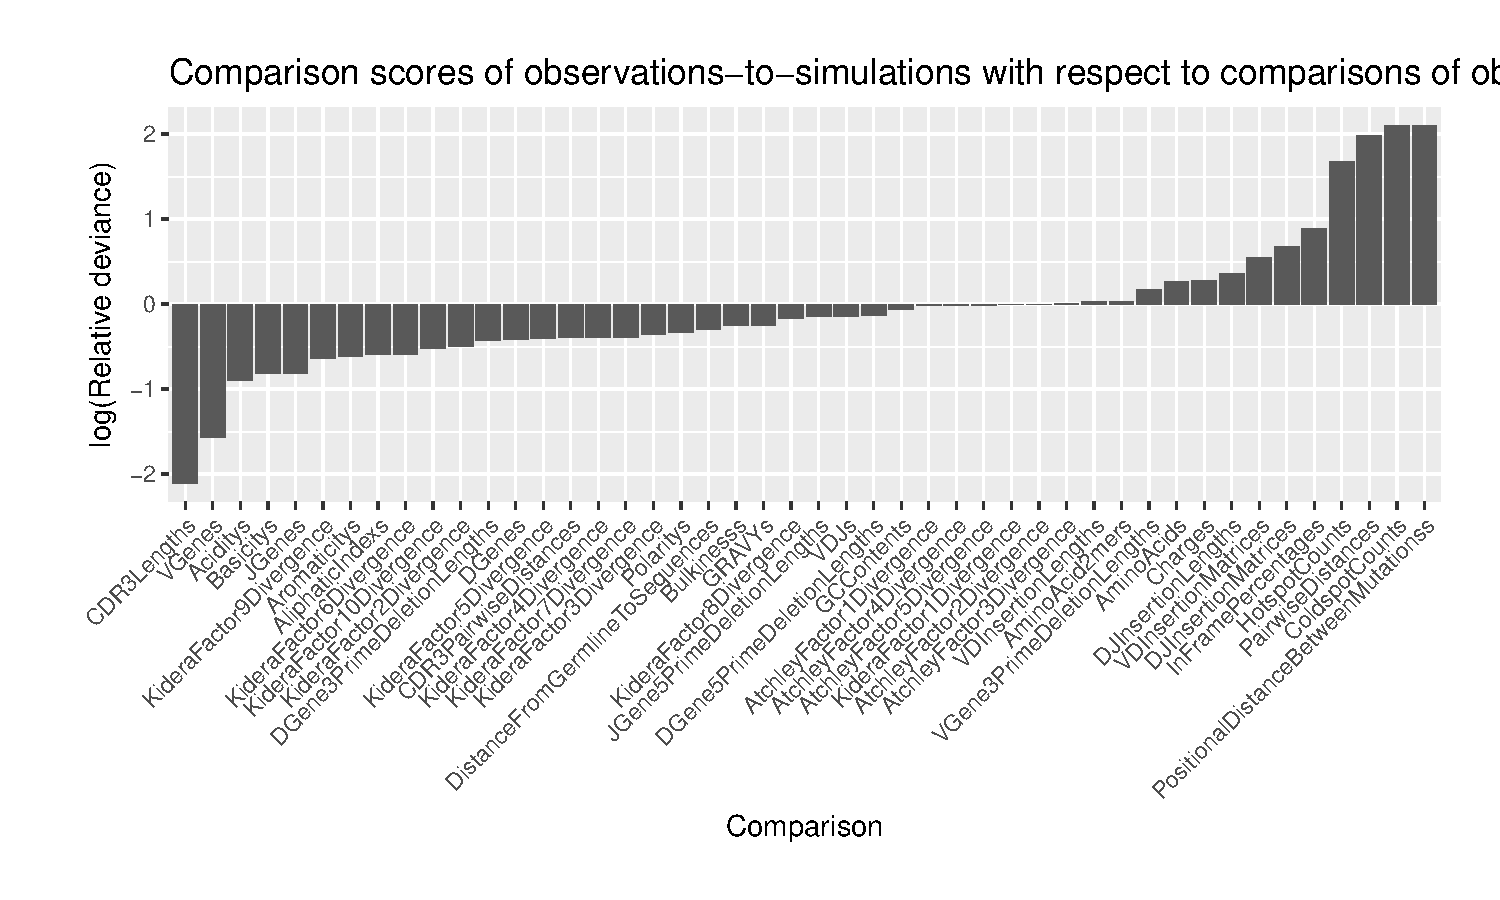
\includegraphics[width=\linewidth]{Figures/score_plot.pdf}
    \caption{The log relative deviance (LRD) of each statistic based on \texttt{partis} model inference and simulation.
        A low LRD indicates a well-replicated statistic by the simulations.
    }
    \label{Scores}
\end{figure}

\subsection*{Comparing observations to competing model simulations}

\section*{Discussion}
We aren't talking about pairwise summary statistics such as UniFrac \cite{De_Bourcy2017-pu}.


\bibliographystyle{plain}
\bibliography{main}

\end{document}
